\documentclass[parskip=never,landscape,twocolumn]{scrreprt}
\parindent=0pt

\usepackage[ngerman]{babel}
\usepackage{amsmath}

\usepackage{mathptmx}

\usepackage{graphicx}
\usepackage{amsmath}
\usepackage{caption}
\usepackage{xcolor}

\usepackage{multicol}
\usepackage{geometry}
\geometry{a4paper, top=7mm, left=10mm, right=10mm, bottom=5mm, includefoot}

\usepackage{fancybox}

%enumnummerierung ebene2
\renewcommand{\labelenumii}{\arabic{enumii}}

%itemizeabstände
\usepackage{xpatch}
\xpatchcmd{\itemize}
  {\def\makelabel}
  {	\setlength{\itemsep}{0mm}
 	\setlength{\parskip}{0pt}
  	\setlength{\parsep}{0pt}  
  \def\makelabel}
  {}
  {}
  
  \xpatchcmd{\enumerate}
  {\def\makelabel}
  {	\setlength{\itemsep}{0mm}
 	\setlength{\parskip}{0pt}
  	\setlength{\parsep}{0pt}  
  \def\makelabel}
  {}
  {}
  
  \newcommand{\halfpage}[1]{\begin{minipage}{0.49\textwidth} #1 \end{minipage}}

\usepackage{amssymb}
\usepackage{tikz}
\usetikzlibrary{shapes}
\usetikzlibrary{trees}
\usetikzlibrary{arrows}

\definecolor{darkgreen}{rgb}{0.1,0.65,0.1}
\definecolor{darkblue}{rgb}{0.1,0.1,0.8}

\newcommand{\minpurp}[1]{\textbf{\textcolor{purple}{ #1}}~\\}
\newcommand{\minmeth}[1]{\textcolor{darkgreen}{\textbf{#1}:~\\}}
\newcommand{\submeth}[1]{\textcolor{darkblue}{\textit{#1}:~}}

\newcommand{\quarterpage}[1]{\begin{minipage}{0.25\textwidth} #1 \end{minipage}}
%\renewcommand{\halfpage}[1]{\begin{minipage}[t]{0.49\textwidth} #1 \end{minipage}}
\begin{document}
%\minpurp{Grundlagen}
%\begin{itemize}
%\item Universalität (muss Turing mächtig sein)
%\item Implementierbarkeit: Korrekte Programme müssen ausgeführt werden können.
%\item Syntax: Form (Anordnung von Zeichen, Ausdrücken...)
% \item Semantik: Bedeutung (Verhalten)
% \item Pragmatik: Zweck (wie, von wem, wozu wird Sprache verwendet)
%\end{itemize}
%\minpurp{Kategorien}
%\submeth{imperativ}
%\begin{itemize}
%\item prozedural z.B. C
%\item objektorientiert z.B. Java, C\#
%\item Skriptsprachen (interpretierbar, dyn. typisiert) z.B. JavaScript, Python
%\end{itemize}
%\submeth{deklarativ}
%\begin{itemize}
%\item funktional z.B. LISP, Scala
%\item logisch z.B. Prolog
%\item Domain Specific Language (DSL) z.B.  SQL, XAML
%\end{itemize}
%
%

\minpurp{Kompilierzeitpunkt}
\minmeth{Früh}Vorteil: Leistungsfähigere Geräte, 1x Übersetzen spart Ressourcen\\
aber: Information über Zielplattform nötig

\submeth{AOT (Ahead-of-Time)} Entwicklung, Server/Store, Installation

\minmeth{Spät}Vorteil: geht immer, einfacherer Compiler/Interpreter, besserer Code möglich da vollständige Information über Hardware, OS, Bibliotheken etc.

\submeth{JIT (Just-in-Time)} Direkt vor/während Ablauf\\
Ablauf: AOT in Zwischencode für hypothetische Maschine (Aufwändige Schritte wie Syntaxanalyse, Typprüfung)\\
JIT von Zwischencode in optimierten Maschinencode => Performanter als Interpreter, Leichtere Validierung, i.d.R. verzögerter Start

\newcommand{\process}[1]{$\rightarrow$ \textcolor{orange}{\textit{#1}}$\rightarrow$\\}
\newcommand{\optprocess}[1]{$\rightarrow$ \textcolor{lightgray}{\textit{#1}}$\rightarrow$\\}
\newcommand{\object}[1]{\textcolor{darkblue}{\textit{#1}~}}
\newcommand{\optobject}[1]{ \textcolor{lightgray}{\textit{#1}}}

\minpurp{Kompiliervorgang}
\object{Zeichenstrom}
\process{Scanner (Lexikalische Analyse} 
\object{Token-Strom}
\process{Parser}	
$\left. 
\begin{minipage}{0.39\textwidth}
  \optobject{Ableitungsbaum}
  \process{AST Generierung \& Semantische Analyse}
  \object{Abstract Syntax Tree (AST)}
  \optprocess{Zwischencode generieren/optimieren} 
  \optobject{Zwischencode}
  \process{Maschinencodegenerierung}
  \object{Maschinencode}
  $\leftrightarrow$ \textcolor{lightgray}{\textit{Maschinencodeoptimierung}}
  \end{minipage} \right\rbrace$
{Symboltabelle}

\minmeth{Scanner}
Erkennt Token für Parser (Schlüsselwörter, Bezeichner, Zahlen,$\dots$) \\
Whitespaces, Kommentare, Präprozessoranweisungen,.. beeinflussen Tokenerkennung

Implementierung: Angepasster DFA (Neustart nach Token, erkennt längstes Mögliches Token, Schlüsselworttabelle, Fehler wenn weder passende Kante noch Endzustand)
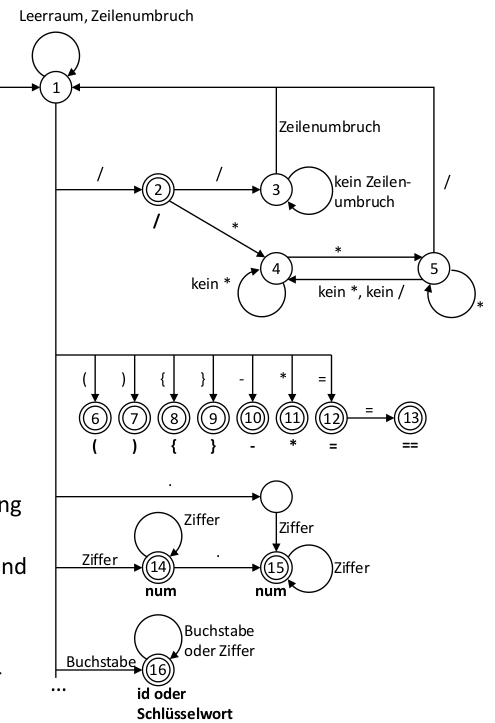
\includegraphics[angle=90,width=0.35\textwidth]{scanner}
\newcommand{\K}{ \textcolor{red}{k} }
\minmeth{Parser}
Rekonstruiert Ableitungsbaum (bzw. den reduzierten AST) gemäß der Grammatik der Programmiersprache.
\begin{itemize}
\item LL(\K) (Links-nach-Rechts Linksableitung); Vorschau von \K Zeichen (v.a. \K = 1)\\ 
		Parsen Top-Down: \\
		Start: Keller enthält Startwort\\
		Ende: Keller und Eingabe sind leer ($\epsilon$)
	\begin{enumerate}
		\item Predict: betrachte die vordersten \K Zeichen und wähle \textbf{die} passende Regel aus der Grammatik.
		\item Match: Entferne übereinstimmende Terminale aus dem Keller und der Eingabe.
	\end{enumerate}
	
	
\item LR (Links-nach-Rechts Rechtsableitung); mächtiger als LL Parser\\
	Parsen Bottom-Up:\\
		Start: Keller ist leer ($\epsilon$)\\
		Ende: Startsymbol im Keller, Eingabe leer
	\begin{enumerate}
		\item Shift: Lade nächstes Zeichen in den Keller
		\item Reduce: wende wenn möglich eine Regel der Grammatik an.
	\end{enumerate}
		

\end{itemize}


\minmeth{Semantische Analyse}
Statische Bindungen (Bezeichner-Objekt $\rightarrow$ Typ-Objekt)$\Rightarrow$ Symboltabelle und AST

\submeth{Symboltabelle} Sammelt Definitionen/Deklarationen von Objekten und damit auch:

\underline{Objektarten}: Namensraum, Typ, Methode/Funktion, Parameter, Variable, Konstante

\underline{Bindungen}: Typ, Adresse, Sichtbarkeit, innerer Gültigkeitsbereich

Gültigkeitsbereiche als Baumstruktur, Mehrdeutige Namen als eindeutiges Symbol


\minmeth{AST}
Reduzierter Ableitungsbaum: 
\begin{itemize}
	\item keine Satzzeichen (desugaring)
	\item Operation Elternknoten, Operanden Kinder
	\item Verkettung der Anweisungen
	\item Deklarationen in Symboltabelle
	\item Namen verweisen auf die Symboltabelle
\end{itemize}

\submeth{Typprüfung}
Typen werden im AST propagiert 
\begin{itemize}
\item Typprüfung
\item Typinferenz (fehlende Typen in Symboltabelle eintragen)
\item Auflösen von Überladungen und Literalen Konstanten
\item implizite Konversionen erkennen
\item generische Typen instanziieren
\end{itemize}



\minmeth{Zwischencode}
Ableitungsbaum - Transpiler (Source-to-Source)

AST - "Lowering": Neue Konstrukte durch alte darstellen (z.B. Iteratoren)

Maschinenunabhängige Optimierung z.B. Function Inlining, Simple constant propagation, loop-unroll, ...



\minmeth{Maschinencode}
Symboltabelle um Adressen erweitern (auch Stackpointer relative)

Registerallokation, Auswahl und Anordnung von Befehlen

\submeth{Maschinenabhängige Optimierung}
Architekturabhängige Befehle/Adressierungen

Cache Coherence

Keyhole-Optimierung: Folgen von Befehlen durch schnellere ersetzen (z.B. *4 durch shift-left 2)

\minmeth{Linken}
statisch: Bibliotheken u. Laufzeitsystem nach Kompilieren => werden in die Binary gepack

dynamisch: Bibliotheken/Laufzeitsystem sind seperat und werden vor ausführung vom Linking Loader im RAM gebunden


\minmeth{Laufzeitsystem}
Zur Ausführung nötiger Code (der Sprache) z.B. für:

Code-Verifikation, JIT, Exceptions, Garbage-Collector, Linken zur Laufzeit

\minpurp{Exceptions}
Ersatz von Fehlercode-Rückgabewerten durch Exceptions;

Implementierung: Tabellen im globalen datensegment ordnen Programmzählerbereiche entsprechenden Handlern zu; 

Stack unwinding: nach werfen der Exception wird stack nach unten durchlaufen bis fehler behandelt


\minpurp{Bindungen}
%Namensbindung, Typbindung, Wertbindung, Adressbindung
%
%anonym vs Namensbindung
%
\submeth{statisch} zur Kompilezeit in Symboltabelle

z.B. int i = 32;  
Achtung: auch Typinferenz (var in C\#)

\submeth{dynamisch} zur Laufzeit im Speicher z.B. Werte, virtuelle Methoden, Typen

z.B. Javascript, dynamic in C\# 

=> Ducktyping

%\minpurp{scope}
%lexikalischer Scope: bindung an den umgebenden Block.
%
%freie Variablen: keine lokale bindung (nicht in diesem Block)
%Funktionen sind Closures wenn alle freien Variablen nicht-lokal gebunden sind
%


\end{document}